\begin{frame}[allowframebreaks,allowdisplaybreaks]
    \subsection{Properties}
    \subsubsection{The \(\alpha\) Constant}
    \frametitle{B-Tree Properties---The \(\alpha\) constant}
    \begin{columns}
        \begin{column}{\textlecolumn}
            \begin{block}{}
                \begin{itemize}
                    \item The main property of the B-Trees is the \(\alpha\), a predefined constant.
                    \item The \(\alpha\) must be a Natural number, \(\alpha \in \mathbb{N}\) and \(\alpha \geq 2\).
                    \item This constant will determine the interval of keys and sub-trees, in a balanced node. This is called the \emph{Branching factor} of the tree.
                    \item The tree is balanced if they have from \(\alpha + 1\) to \(2\alpha + 1\) sub-trees in a single node.
                    \item Also, each balanced node have from \(\alpha\) to \(2\alpha\) keys.
                    \item The only node that can have less than \(\alpha + 1\) sub-trees and only 1 key is the \emph{Root} of the tree. 
                    \item But, the \emph{Root} still have the upper bounds of sub-trees and keys.
                \end{itemize}
            \end{block}
        \end{column}
        \begin{column}{\textricolumn}
        \end{column}
    \end{columns}
    \begin{columns}
        \begin{column}{0.5\textwidth}
                \begin{figure}
                    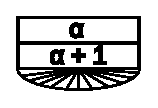
\includegraphics[width=0.45\textwidth]{resources/made/min_node.eps}
                    \caption[]{Miminum Keys and Sub-Trees on a Node}
                \end{figure}
        \end{column}
        \begin{column}{0.5\textwidth}

                \begin{figure}
                    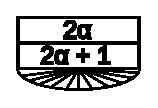
\includegraphics[width=0.45\textwidth]{resources/made/max_node.eps}
                    \caption[]{Maximun Keys and Sub-Trees on a Node}
                \end{figure}
        \end{column}
    \end{columns}
    
    \framebreak{}

    \begin{figure}
        \centering
        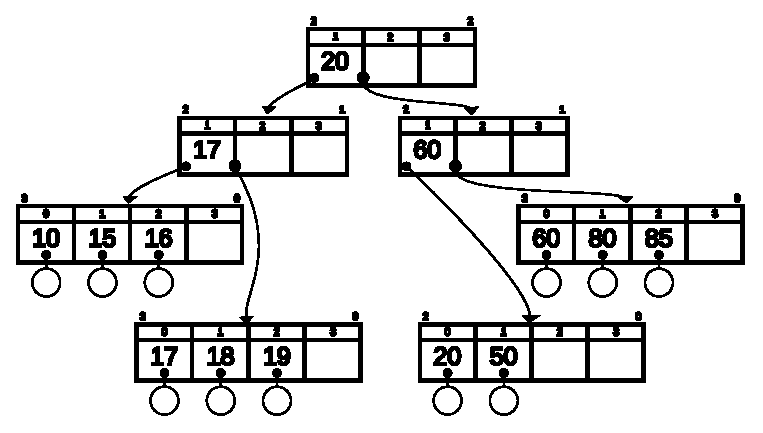
\includegraphics[width=0.95\linewidth,keepaspectratio]{resources/made/mendivelso_a2_btree.eps}
        \caption[]{B-Tree, t (2, 2)}
    \end{figure}

    \framebreak{}

    \begin{columns}
        \begin{column}{\textlecolumn}
            \begin{block}{}
                \vspace{-0.5cm}
                \begin{itemize}
                    \item We can prove the bounds of the number of sub-trees in a node, and define a function that let us get the number of sub-trees in a node.
                \end{itemize}
            \end{block}
        \end{column}
        \begin{column}{\textricolumn}
        \end{column}
    \end{columns}
    \begin{columns}
        \begin{column}{0.45\textwidth}
            \begin{block}{}
                \begin{proof}\renewcommand{\qedsymbol}{}
                    Let \(T \in t\left(\alpha, h\right)\), and \(N(T)\) be a function that returns the number of nodes in \(T\).
                    Let \(N_{\text{min}}\) and \(N_{\text{max}}\) the minimum and maximal number of nodes in \(T\). Then
                    \[
                        \begin{aligned}
                            N_{\text{min}} &= 1 + 2\left(\left(\alpha + 1\right){}^0 + \left(\alpha + 1\right){}^1 + \cdots + \left(\alpha + 1\right){}^{h-2} \right) \\
                            & = 1 + 2\left(\sum^{h - 2}_{i = 0} \left(\alpha + 1\right){}^i \right) \\
                            & = 1 + \frac{2}{\alpha}\left(\left(\alpha + 1\right){}^{h - 1} - 1\right)
                        \end{aligned}
                    \]
                \end{proof}
            \end{block}
        \end{column}
        \begin{column}{0.6\textwidth}
            \begin{figure}
                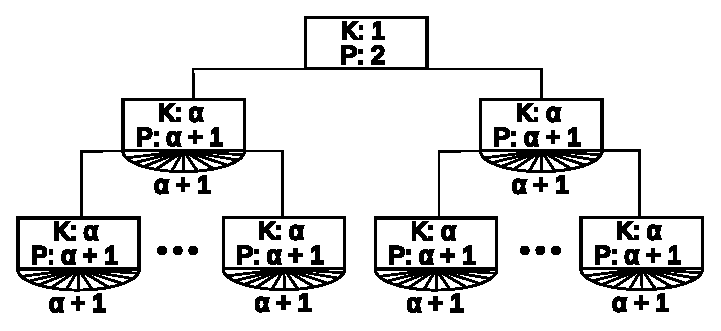
\includegraphics[width=\linewidth,keepaspectratio]{resources/made/generic_min_btree.eps}
                \caption[]{B-Tree w/ the least number of nodes}
            \end{figure}
        \end{column}
    \end{columns}

    \framebreak{}

    \begin{columns}
        \begin{column}{0.4\textwidth}
            \begin{block}{}
                \begin{proof}[\unskip\nopunct]\renewcommand{\qedsymbol}{}
                    For \(h \geq 1\), we also have that
                    \[
                        \begin{aligned}
                            N_{\text{max}} &= 2\left(\sum^{h - 1}_{i = 0} \left(2\alpha + 1\right){}^i \right) \\
                            &= \frac{1}{2\alpha}\left(\left(2\alpha + 1\right){}^{h} - 1\right) \\
                        \end{aligned}
                    \]
                \end{proof}
            \end{block}
        \end{column}
        \begin{column}{0.6\textwidth}
            \begin{figure}
                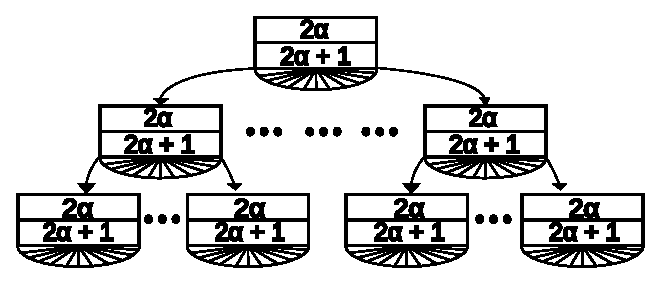
\includegraphics[width=1\linewidth,keepaspectratio]{resources/made/generic_max_btree.eps}
                \caption[]{B-Tree w/ the most number of nodes}
            \end{figure}
        \end{column}
    \end{columns}
    \begin{columns}
        \begin{column}{\textlecolumn}
            \begin{block}{}
                \begin{proof}[\unskip\nopunct]
                    Then, if \(h = 0\), we have that \(N\left(T\right) = 0\). Else, if \(h \geq 1\)
                    \[
                        1 + \frac{2}{\alpha}\left(\left(\alpha + 1\right){}^{h - 1} - 1\right) 
                        \leq 
                        N\left(T\right) 
                        \leq 
                        \frac{1}{2\alpha}\left(\left(2\alpha + 1\right){}^{h} - 1\right)
                        \tag{Nodes Bounds}\label{btree-nodes-num}
                    \]
                \end{proof}
            \end{block}
        \end{column}
        \begin{column}{\textricolumn}
        \end{column}
    \end{columns}

    \framebreak{}

    \begin{columns}
        \begin{column}{\textlecolumn}
            \begin{block}{}
                \begin{itemize}
                    \item Keep in mind that the \emph{Branching Factor} of a B-Tree might change from each implementation, mostly in papers and books.
                    \item For example, on the original paper by Bayer and McCreight of B-Trees\cite{bayer_organization_1972}, the \emph{Branching Factor} 
                        goes from \(\alpha + 1\) to \(2\alpha + 1\) subtrees and from \(\alpha\) to \(2\alpha\) keys on a node.
                    \item But in the book made by Brass\cite{brass_advanced_2008}, the \emph{Branching Factor} goes from 
                        \(\alpha\) to \(2\alpha - 1\) for both, subtrees and keys in a node.
                    \item And on the original paper by Huddleston and Mehlhorn of AB-Trees\cite{huddleston_new_1982} keeps the same \emph{Branching Factor} as Brass.
                    \item But, we will see later that by limiting the upper bound of the \emph{Branching Factor} to something greater than \(2\alpha\) 
                        we will reach a even greater performance from this type of data structure.
                \end{itemize}
            \end{block}
        \end{column}
        \begin{column}{\textricolumn}
        \end{column}
    \end{columns}

\end{frame}
